\documentclass[10pt,a4paper]{style}

%%%%%%%%% Preamble

% used for figures:
\usepackage{graphicx}
% math fonts etc.:
\usepackage{amsmath,amsfonts,amsthm,latexsym,amssymb}
\usepackage{pdfpages}
\usepackage{caption,subcaption}
\captionsetup[figure]{font=small,labelfont=small}
\usepackage{hyperref}
\hypersetup{
	colorlinks,
	citecolor=black,
	filecolor=black,
	linkcolor=blue,
	urlcolor=black
}
\usepackage{wrapfig}
\setlength\intextsep{2pt} % avoid too much space around figure (can be set to 0pt at maximum)

\graphicspath{ {figures/} }
\usepackage{multicol}

%%%%%%%%%%

\begin{document}
	\tableofcontents
	\listoffigures
	\newpage
	\begin{center}
		\textcolor{orange}{\Large {\bf{Thera Bank Credit Card Service}}}
	\end{center}
	
	\section{Business context}
	The Thera bank recently saw a steep decline in the number of users of their credit card, credit cards are a good source of income for banks because of different kinds of fees charged by the banks like annual fees, balance transfer fees, and cash advance fees, late payment fees, foreign transaction fees, and others. Some fees are charged to every user irrespective of usage, while others are charged under specified circumstances.
	
	Customers’ leaving credit card services would lead the bank to loss. By leveraging data-driven insights, Thera Bank can enhance its credit card services, address customer concerns, and ultimately reduce the rate of attrition. This proactive approach not only helps in retaining existing customers but also strengthens the bank's competitive position in the market.
	
\section{Exploratory Data Analysis}
\subsection{Data set description}
	\begin{figure}[h]
		\centering
		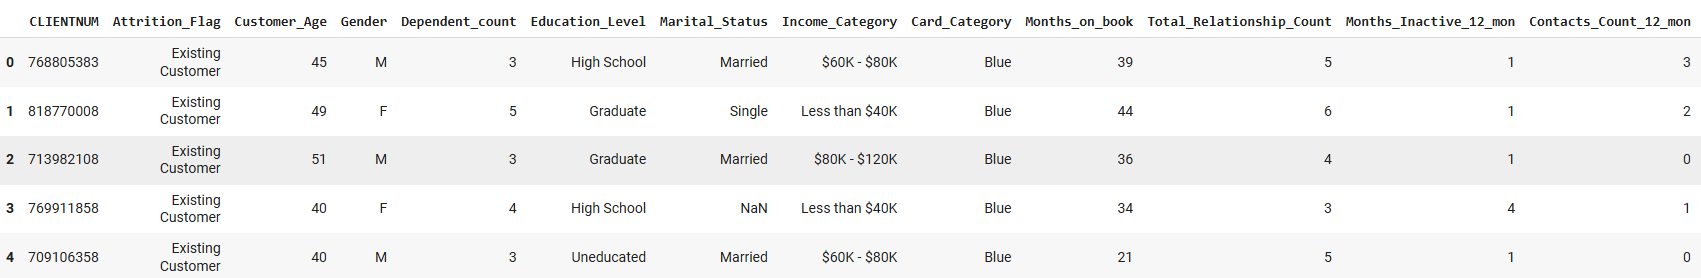
\includegraphics[width=\textwidth]{dataset.png}
		\caption{A snapshot of data set used for analysis.}
		\label{fig:dataset}
	\end{figure}
We have been provided with a dataset consisting of Ther Bank's customer's credit card usage details and also with some of their background with the target field of whether the customer has attrited/inactive. The details of each field is described as follows:

CLIENTNUM: Client number. Unique identifier for the customer holding the account.
Attrition\_Flag: Internal event (customer activity) variable - if the account is closed then "Attrited Customer" else "Existing Customer".
Customer\_Age: Age in years.
Gender: Gender of the account holder.
Dependent\_count: Number of dependents.
Education\_Level: Educational qualification of the account holder - Graduate, High School, Unknown, Uneducated, College (refers to college student), Post-Graduate, Doctorate.
Marital\_Status: Marital status of the account holder.
Income\_Category: Annual income category of the account holder.
Card\_Category: Type of card.
Months\_on\_book: Period of relationship with the bank (in months).
Total\_Relationship\_Count: Total number of products held by the customer.
Months\_Inactive\_12\_mon: Number of months inactive in the last 12 months.
Contacts\_Count\_12\_mon: Number of contacts in the last 12 months.
Credit\_Limit: Credit limit on the credit card.
Total\_Revolving\_Bal: Total revolving balance on the credit card. This represents the balance that carries over from one month to the next on a credit card. It's the amount that remains unpaid at the end of the billing cycle and is carried forward to the next month.
Avg\_Open\_To\_Buy: Open to buy credit line (average of last 12 months). This is the average amount of credit available to use on the credit card over the last 12 months. It indicates how much credit is left after accounting for the current balance.
Total\_Amt\_Chng\_Q4\_Q1: Change in transaction amount (Q4 over Q1). This is the ratio of the total transaction amount in the 4th quarter to the total transaction amount in the 1st quarter. It indicates how the transaction amount has changed between these two periods.
Total\_Trans\_Amt: Total transaction amount (last 12 months). This is the total amount of all transactions made using the credit card over the last 12 months. It includes all purchases, payments, and other transactions.
Total\_Trans\_Ct: Total transaction count (last 12 months). This is the total count of all transactions made using the credit card over the last 12 months. It reflects the frequency of card usage.
Total\_Ct\_Chng\_Q4\_Q1: Change in transaction count (Q4 over Q1). This is the ratio of the total transaction amount in the 4th quarter to the total transaction amount in the 1st quarter. It indicates how the transaction amount has changed between these two periods.
Avg\_Utilization\_Ratio: Average card utilization ratio. This represents the average utilization of the available credit over a period. It shows how much of the available credit the customer has used, on average. There are total 21 columns or fields. CLIENTNUM consists of unique IDs for clients and hence will not add value to the modeling. Therefore we have dropped it from our analysis. Total number of rows are 10,127 among which we did not find any duplicated records in the data set. But there were some irregular and missing values in the data set which We will describe in the data preprocessing section. Let's proceed to exploratory analysis with basic plots which will give us important insights.

\subsection{Exploratory analysis}	
As shown in figure \ref{fig:Categorical variable profile} We have plotted distribution in various categorival variable. We observe that the whole data set has an attrition rate of around 16 \%. There are various groups of income level. Less than 40K category has highest percentage of customers as shown in \ref{fig:Income_Category}. The 'abc' value has been treated appropriately before the model building. Most of the customers have dependents on them with 2 and 3 being higher mode as shown in figure \ref{fig:Dependent_count}. Among the various available credit card types, 'Blue' is the most preferred one. Gold, Platinum an Silver are used very scarcely, figure \ref{fig:Card_Category}. More than 85 \% of customers have some form of education with lowest being high school and highest being a doctorate. 1487 did not have any education as shown in figure \ref{fig:Education_Level}. There are around 400 customer who did not have any contact with the bank in last 12 months. More than 85\% of customers have  at least 2 contacts with the bank in last 12 months, figure \ref{fig:Contacts_Count_12_mon}. 
	\begin{figure}[h]
		\centering
		\begin{subfigure}[t]{0.3\textwidth}
			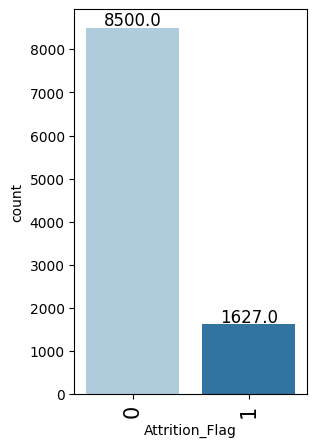
\includegraphics[width=\textwidth,height=6cm]{Attrition_Flag.png}
			\caption{Attrition Rate in our dataset.}
			\label{fig:Attrition_Flag}
		\end{subfigure}
		\hfill
		\begin{subfigure}[t]{0.3\textwidth}
			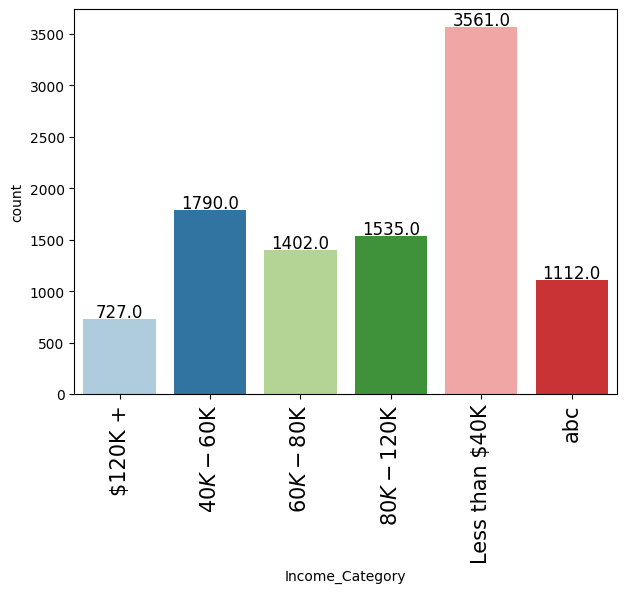
\includegraphics[width=\textwidth,height=6cm]{Income_Category.png}
			\caption{Income distribution in customers.}
			\label{fig:Income_Category}
		\end{subfigure}
		\hfill
		\begin{subfigure}[t]{0.3\textwidth}
			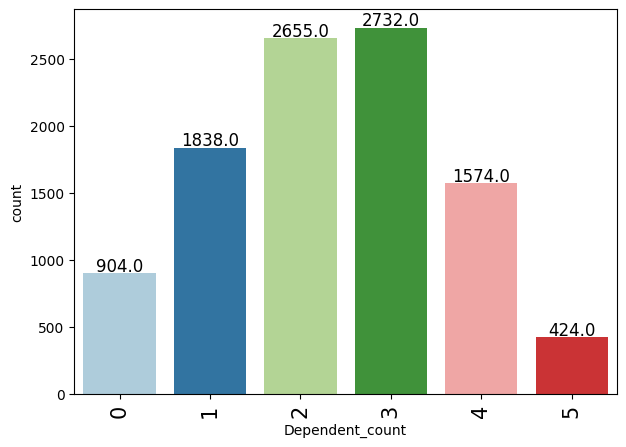
\includegraphics[width=\textwidth,height=6cm]{Dependent_count.png}
			\caption{Dependent count distribution.}
			\label{fig:Dependent_count}
		\end{subfigure}
		\hfill
		\begin{subfigure}[t]{0.3\textwidth}
			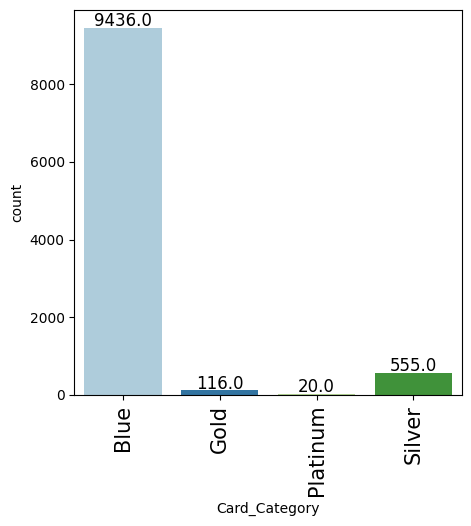
\includegraphics[width=\textwidth,height=6cm]{Card_Category.png}
			\caption{preferences over Card Categories.}
			\label{fig:Card_Category}
		\end{subfigure}
		\hfill
		\begin{subfigure}[t]{0.3\textwidth}
			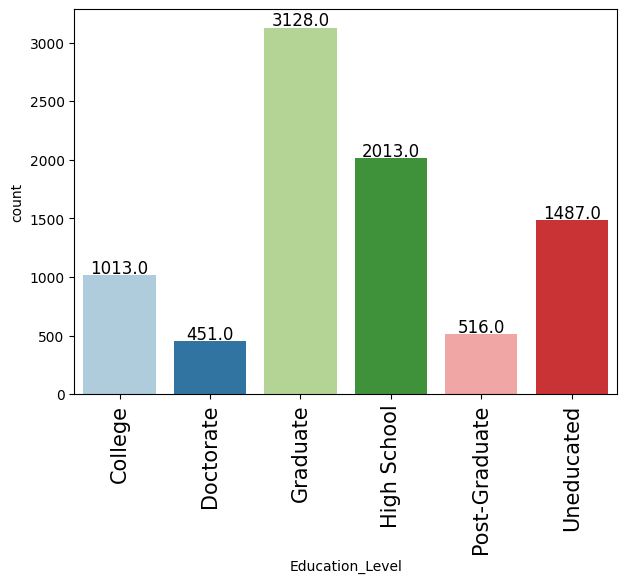
\includegraphics[width=\textwidth,height=6cm]{Education_Level.png}
			\caption{Education Level background among customers}
			\label{fig:Education_Level}
		\end{subfigure}
		\hfill
		\begin{subfigure}[t]{0.3\textwidth}
			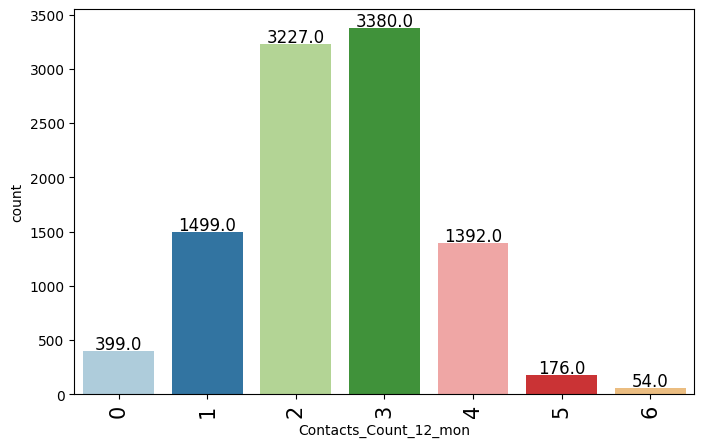
\includegraphics[width=\textwidth,height=6cm]{Contacts_Count_12_mon.png}
			\caption{Contacts Count in last 12 months made by the customers with the bank.}
			\label{fig:Contacts_Count_12_mon}
		\end{subfigure}
		\caption{Profile of Categorical variables.}
		\label{fig:Categorical variable profile}
	\end{figure}
	%%%%%%%%
	Figure \ref{fig:stackplot_wrt_target} shows stacked bar plots of categorical variables with respect to attrition flag of 0 or 1. The stacked bar chart in \ref{fig:Attrition_Flag vs Total_Relationship_Count} illustrates the distribution of two categories (0 and 1) across different values of "Total\_Relationship\_Count." The x-axis represents the "Total\_Relationship\_Count" with values ranging from 1 to 6, while the y-axis shows the proportion of each category, ranging from 0 to 1. The blue segments represent category 0, and the orange segments represent category 1. "Total\_Relationship\_Count" increases, the proportion of category 0 (blue) generally increases, while the proportion of category 1 (orange) decreases. Customers with higher "Total\_Relationship\_Count" (values 5 and 6) are predominantly in category 0, indicating that customers with more products held are less likely to attrition. Conversely, customers with fewer products are more likely to attrition. 
	The chart on "\ref{fig:Attrition_Flag vs Months_Inactive_12_mon} illustrates the distribution of two categories (0 and 1) across different values of "Months\_Inactive\_12\_mon. This plot  is little bit deceiving as the pattern is bit mixed. Although customers with no inactive months are more likely to attrition but in our data set there are very few such customers. Among 1,2 and 3 which has highest frequencies, the pattern is more clear. The attrition rate increases from 1 to 3. 
	The chart on \ref{fig:Attrition_Flag vs Contacts_Count_12_mon} illustrates the distribution of two categories (0 and 1) across different counts of contacts in the last 12 months (Contacts\_Count\_12\_mon). Here the pattern is quite clear. Customers with higher contact counts (values3, 4, 5 and 6) have higher portion in category 1, indicating that more frequent contact is associated with attrition category. In fact the customers(total 54) who have contacted 6 times last year have all attrited.    
	\begin{figure}[h]
		\centering
		\begin{subfigure}[t]{0.32\textwidth}
			\centering
			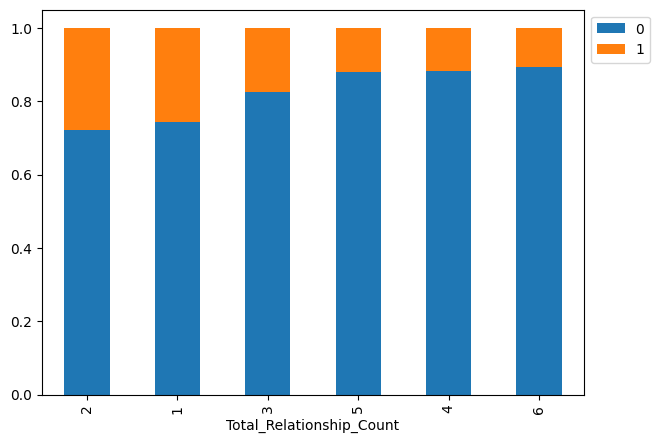
\includegraphics[width=\textwidth,height=5cm]{Attrition_Flag vs Total_Relationship_Count.png}
			\caption{}
			\label{fig:Attrition_Flag vs Total_Relationship_Count}
		\end{subfigure}
		\hfill
		\begin{subfigure}[t]{0.32\textwidth}
			\centering
			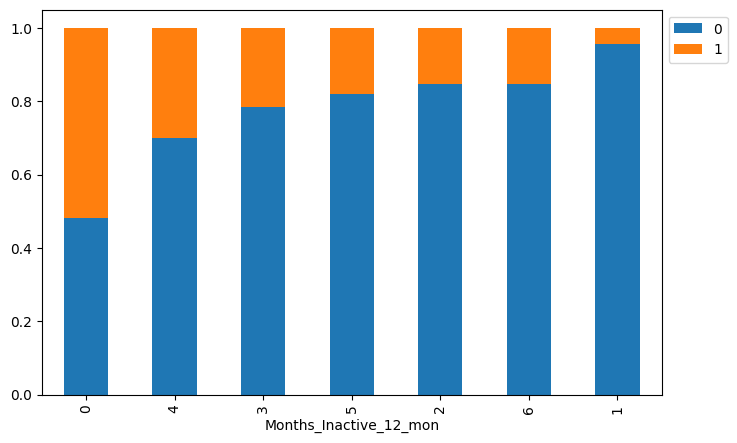
\includegraphics[width=\textwidth,height=5cm]{Attrition_Flag vs Months_Inactive_12_mon.png}
			\caption{}
			\label{fig:Attrition_Flag vs Months_Inactive_12_mon}
		\end{subfigure}
		\hfill
		\begin{subfigure}[t]{0.32\textwidth}
			\centering
			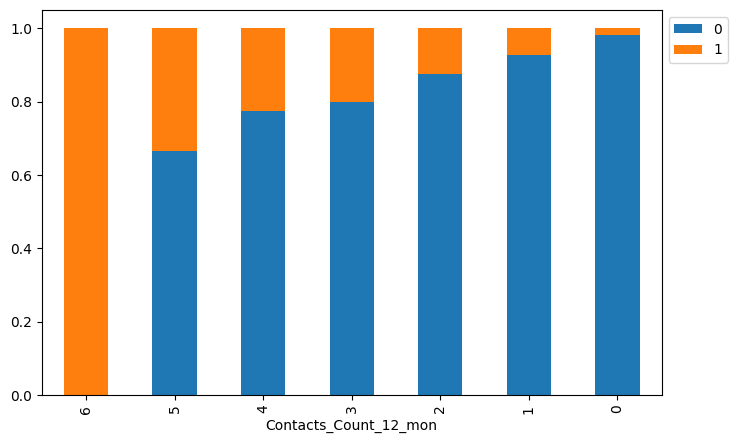
\includegraphics[width=\textwidth,height=5cm]{Attrition_Flag vs Contacts_Count_12_mon.png}
			\caption{}
			\label{fig:Attrition_Flag vs Contacts_Count_12_mon}
		\end{subfigure}
		\hfill
		\begin{subfigure}[t]{0.32\textwidth}
			\centering
			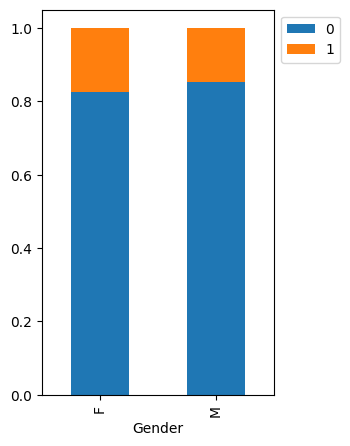
\includegraphics[width=\textwidth,height=5cm]{Attrition_Flag vs Gender.png}
			\caption{}
			\label{fig:Attrition_Flag vs Gender}
		\end{subfigure}
		\hfill
		\begin{subfigure}[t]{0.32\textwidth}
			\centering
			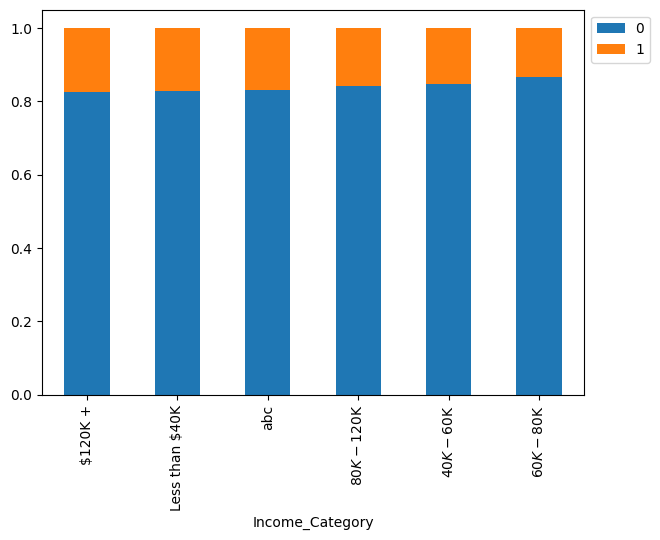
\includegraphics[width=\textwidth]{Attrition_Flag vs Income_Category.png}
			\caption{}
			\label{fig:Attrition_Flag vs Income_Category}
		\end{subfigure}
		\hfill
		\begin{subfigure}[t]{0.33\textwidth}
			\centering
			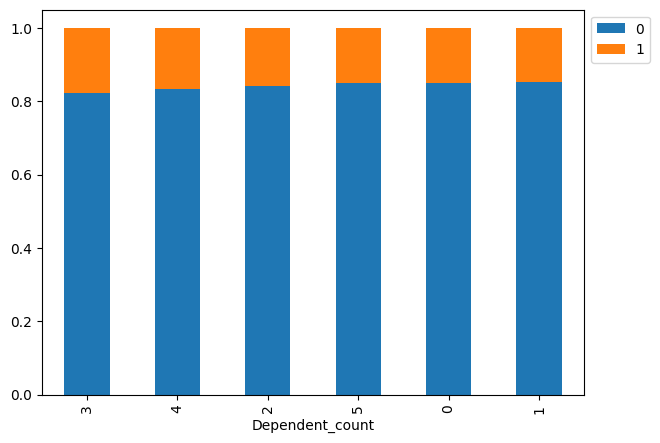
\includegraphics[width=\textwidth,height=5cm]{Attrition_Flag vs Dependent_count.png}
			\caption{}
			\label{fig:Attrition_Flag vs Dependent_count}
		\end{subfigure}
		\caption{Normalized stack plot distribution of categorical variables with respect target.}
		\label{fig:stackplot_wrt_target}
	\end{figure}
		Similar charts on figure \ref{fig:Attrition_Flag vs Gender}, \ref{fig:Attrition_Flag vs Income_Category}, \ref{fig:Attrition_Flag vs Dependent_count} shows the attrition prevalence with respect to gender, income category and Dependent count. In these the differences are not significantly pronounced. Yet it is worth while to note that Females have slightly higher attrition ratio and the high earners ( more than 120K ) and low earners (less than 40K) have slightly higher attrition ratio.  
	\begin{figure}[h]
		\centering
		\begin{subfigure}[t]{0.47\linewidth}
			\centering
			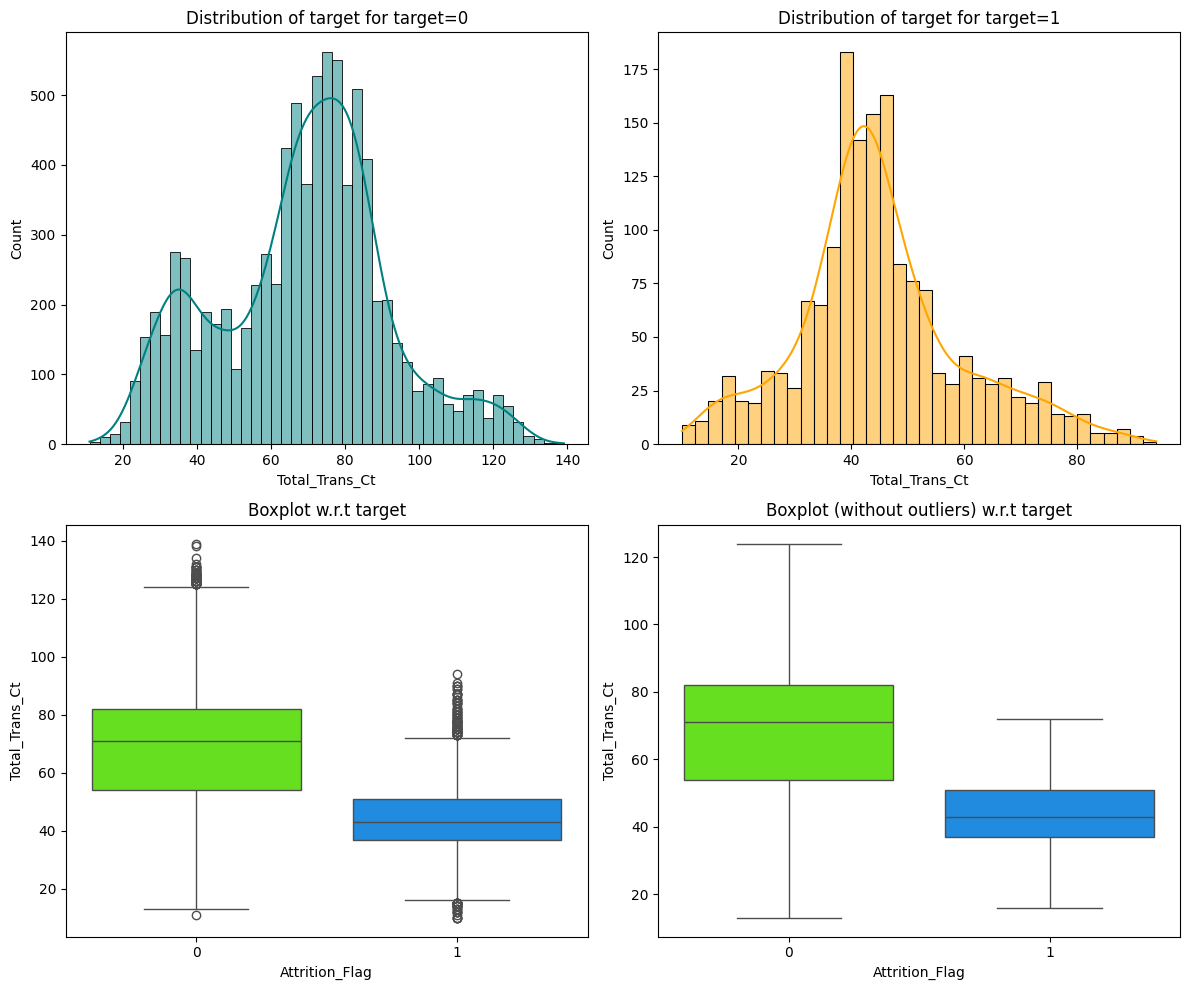
\includegraphics[width=\linewidth]{Total_Trans_Ct vs Attrition_Flag.png}
			\caption{Histogram and boxplot of Total transaction count w.r.t attrition flag}
			\label{fig:Total_Trans_Ct vs Attrition_Flag}
		\end{subfigure}
		\hfill
		\begin{subfigure}[t]{0.47\linewidth}
			\centering
			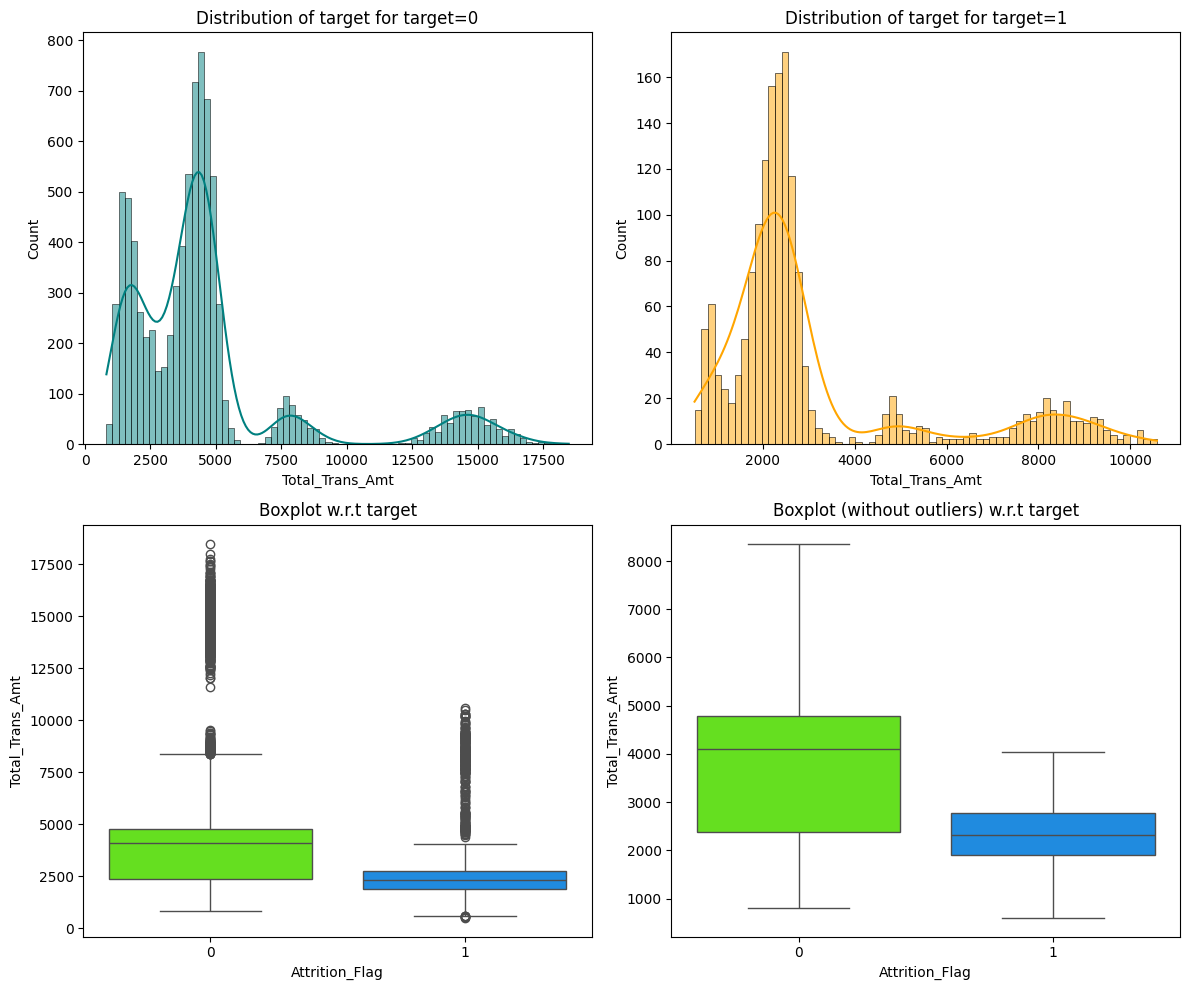
\includegraphics[width=\linewidth]{Total_Trans_Amt vs Attrition_Flag.png}
			\caption{Histogram and boxplot Total transaction amount w.r.t attrition flag}
			\label{fig:Total_Trans_Amt vs Attrition_Flag}
		\end{subfigure}
		\hfill
		\begin{subfigure}[t]{0.47\linewidth}
			\centering
			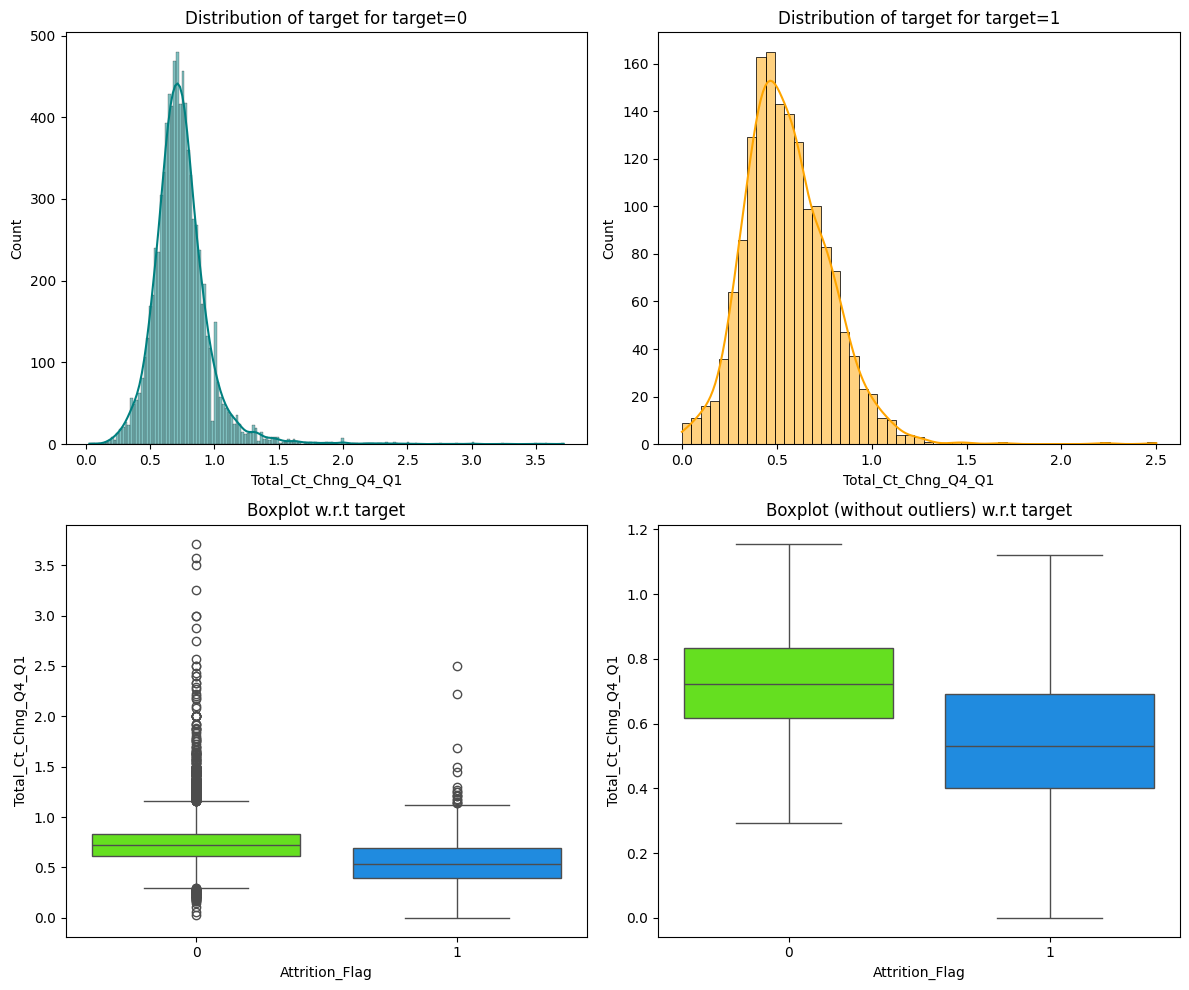
\includegraphics[width=\linewidth]{Total_Ct_Chng_Q4_Q1 vs Attrition_Flag.png}
			\caption{Histogram and boxplot of transaction count change ratio from Q4 to Q1 w.r.t attrition flag}
			\label{fig:Total_Ct_Chng_Q4_Q1 vs Attrition_Flag}
		\end{subfigure}
		\hfill
		\begin{subfigure}[t]{0.47\linewidth}
			\centering
			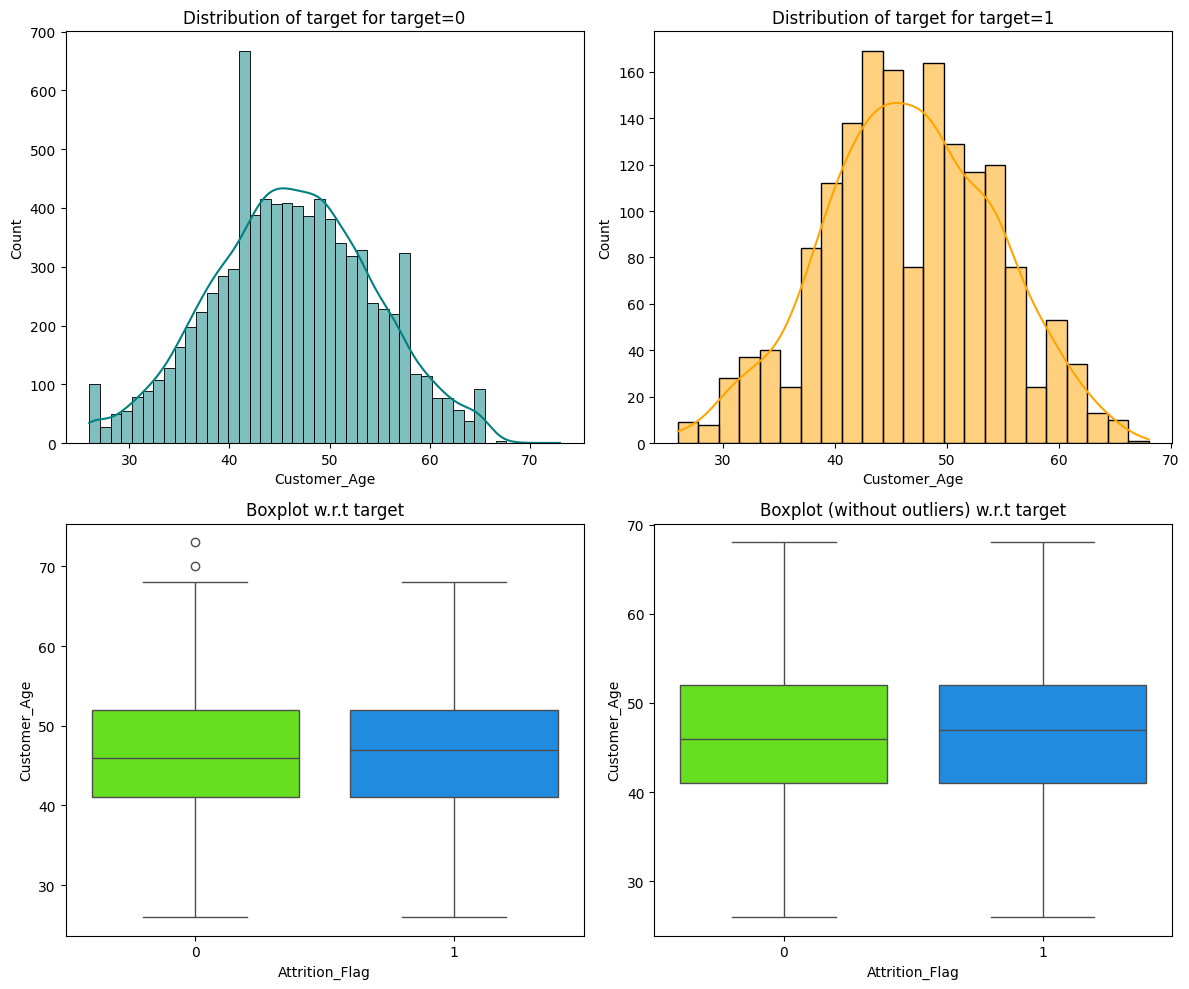
\includegraphics[width=\linewidth]{Attrition_Flag vs Customer_Age.png}
			\caption{Histogram and boxplot customer age w.r.t attrition flag}
			\label{fig:Attrition_Flag vs Customer_Age}
		\end{subfigure}
		\caption{Distribution of numerical variables with respect attrition flag}
		\label{fig: Distribution of numerical variables with respect attrition flag}
	\end{figure}
	
	The figure on \ref{fig: Distribution of numerical variables with respect attrition flag} shows distribution of numerical variables with respect to attrition flag. The plot on \ref{fig:Total_Trans_Ct vs Attrition_Flag} consists of four sub plots that analyze the distribution and box plots of the variable "Total\_Trans\_Ct" with respect to the target variable "Attrition\_Flag."  The boxplot on bottom right shows the distribution of "Total\_Trans\_Ct" with respect to the target variable "Attrition\_Flag" without outliers.  The boxplot for target=0  shows a higher median and a wider interquartile range compared to target=1, but without the influence of outliers. This means attrited customers have lower median total transaction count. This same story is also seen in the plot with respect to total transaction amount in figure \ref{fig:Total_Trans_Amt vs Attrition_Flag}. Similarly figure \ref{fig:Total_Ct_Chng_Q4_Q1 vs Attrition_Flag} shows that attrited customers generally have lower ratio of Q4 to Q1 transaction signifying that their transaction amount quarter over quarter has decreased. 
	
\subsection{Data pre-processing}
	There were outliers in numerical variables. Credit Limit field had highest number of outliers, around 9.7 \%. But no action is done on them as all of them are valid data records from the bank. The anomalous values in the income category was replaced with NaN. Then all the NaN/missing values were treated by imputer with strategy as most frequent. This means that the imputer replaced missing values in each column with the most frequent (mode) value of that column. This approach is particularly useful for categorical data, where the most common category can be a reasonable guess for missing values. It helps in maintaining the integrity of the dataset by filling in gaps with the most likely values based on the existing data. But note that before this operation the data set was already partitioned into training, validation and test data sets to avoid any data leakage. Data leakage occurs when information from outside the training dataset is used to create the model, leading to overly optimistic performance estimates. This can happen if data that would not be available at prediction time is included in the training process, such as future data or target labels. To prevent data leakage, it's crucial to carefully separate training and validation datasets and ensure that only information available at prediction time is used during model training. Data transformations should be applied separately to the training and validation sets to avoid inadvertently leaking information from one to the other. Also the categorical field encoding was done separately on each partition. 
	%%%%%%%%%%%%%%%%%%%%%%%%%%%%%%%%%%%%%%%%%%%%%%%%%%%%%%%%%%%%%%%%%%%%%%%%%%
\section{Model Building}
We have tried following models on our data set before hyper parameter tuning:
\begin{itemize}
	\item Bagging Classifier
	\item Random Forest Classifier
	\item Gradient Boosting Classifier
	\item AdaBoost Classifier
	\item Decision Tree Classifier
	\item XGB Classifier
\end{itemize}
Before we describe the implemented models, we should reflect on our motivation behind how we evaluate these models pertaining to the business problem at our hand. make it 150 words
In predicting customer attrition, a model can make two types of errors: predicting a customer will leave when they stay, and predicting a customer will stay when they leave. The latter is more critical for banks, as it involves losing valuable customers. To reduce this loss, the focus should be on minimizing false negatives by maximizing recall. Higher recall means more at-risk customers are correctly identified, allowing the bank to take action to retain them. By prioritizing recall, the bank can better identify and retain customers who are at risk of leaving.

To mitigate this loss, it is essential to focus on reducing false negatives. One effective approach is to maximize the recall of the model. Recall measures the proportion of actual positives (customers who will attrite) that are correctly identified by the model. By increasing recall, the bank can ensure that more at-risk customers are accurately identified, allowing for targeted retention efforts.

As shown in figure \ref{fig:Model Building - Original Data}, let's summarize these model's performance on training and validation set of Original Data. Random forest, Decision tree and XGB performs perfectly and Bagging close to 98\% on the training set. While on the validation set their performances are 79\%, 81\%, 90\% and 81 \% respectively. This shows that theses model are performing in over fit region on original data set. GBM and Adaboost on the other hand are doing better on generalization, Both performing around 85\% on the Validation similar to the training.     
\subsection{Model Building - with over sampling and under sampling}
In classification problems, imbalanced datasets are common, where the minority class is more significant than the majority class. Handling these datasets effectively is crucial for building robust predictive models. Specialized techniques can address this imbalance, ensuring accurate identification of the minority class. Methods like oversampling the minority class, undersampling the majority class, or using algorithms designed for imbalance can improve model performance. By focusing on these techniques, one can develop a predictive model that is both accurate and reliable, even with imbalanced data. This approach ensures that the minority class, often more valuable, is correctly identified and addressed. We have used SMOTE method to build oversampled data set. SMOTE (Synthetic Minority Oversampling TEchnique) synthesizes new elements for the minority class by randomly selecting a point and computing its k-nearest neighbors. Synthetic points are then added between the chosen point and its neighbors, effectively balancing the dataset and improving model performance on imbalanced data. For under sampling we have used Random under sampler which randomly selects a subset of the majority class to match the number of samples in the minority class. 
	\begin{figure}[h]
		\centering
		\begin{subfigure}[t]{0.32\textwidth}
			\centering
			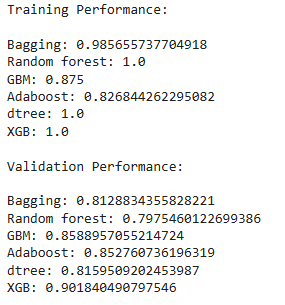
\includegraphics[width=\textwidth,height=6cm]{Model Building - Original Data.png}
			\caption{Model Building performance - Original Data}
			\label{fig:Model Building - Original Data}
		\end{subfigure}
		\hfill
		\begin{subfigure}[t]{0.32\textwidth}
			\centering
			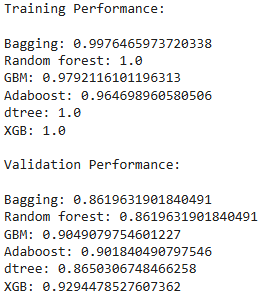
\includegraphics[width=\textwidth,height=6cm]{Model Building - Oversampled Data.png}
			\caption{Model Building performance - Over sampled Data}
			\label{fig:Model Building - Oversampled Data}
		\end{subfigure}
		\hfill
		\begin{subfigure}[t]{0.32\textwidth}
			\centering
			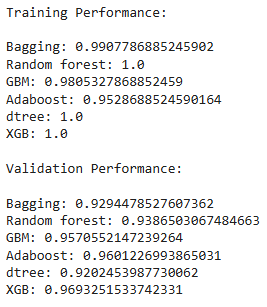
\includegraphics[width=\textwidth,height=6cm]{Model Building - Undersampled Data.png}
			\caption{Model Building performance - Under sampled Data}
			\label{fig:Model Building - Undersampled Data}
		\end{subfigure}
		\caption{Model performance with different sampling.}
		\label{fig:Model performance with different sampling}
	\end{figure}
we observe in figure \ref{fig:Model Building - Oversampled Data} and \ref{fig:Model Building - Undersampled Data} that all the models are performing better on the oversampled and undersampled data set compared to the original data. Also the overfitting issue has improved compared to the original data. Among these we find that XGB is performing with best accuracy of  96.9\% on the undersampled dataset followed by Adaboost with 96\% on the same. 
\subsection{Model Performance Improvement using Hyperparameter Tuning}	
Hyperparameter tuning is the process of optimizing the parameters that control the behavior of a machine learning algorithm. Unlike model parameters, hyperparameters are set before training and influence how the model learns from data. Effective tuning can significantly improve model performance. Techniques like GridSearchCV and RandomizedSearchCV are commonly used to explore different hyperparameter combinations. GridSearchCV exhaustively searches through a specified parameter grid, while RandomizedSearchCV samples a specified number of parameter settings from a distribution. The goal is to find the best hyperparameter values that maximize the model's performance on validation data, ensuring robust and accurate predictions.

In this analysis, we have employed RandomizedSearchCV on the following scenarios:
\begin{multicols}{2}
\begin{itemize}
	\setlength\itemsep{-5pt}
	\item Tuning AdaBoost using original data
	\item Tuning Ada Boost using undersampled data
	\item Tuning Gradient Boosting using undersampled data
\end{itemize}
\columnbreak
\begin{itemize}
	\setlength\itemsep{-5pt}
	\item Tuning Gradient Boosting using original data
	\item Tuning Gradient Boosting using over sampled data
	\item Tuning XGBoost Model with Original data
\end{itemize}
\end{multicols}
\subsection{Model Performance Comparison and Final Model Selection}
	The performance of the tuned models are summarized in figure \ref*{fig:Training performance comparison} and \ref{fig:Validation performance comparison} for four good result scenarios. We see that on the training set all the four tuned models have accuracy greater than 97\%. XGBoost is giving perfect result for recall which brings it into the attention of overfitting. Though compared to the previous models, these tuned models are relatively safer in terms of overfitting as we see that in the validation set these are also performing nicely in terms of accuracy and recall. Gradient Boosting trained with original data shows the highest accuracy, precision, and F1 score, making it highly effective in identifying relevant instances accurately. AdaBoost trained with undersampled data has the highest recall 96.6 \%, indicating it is effective in identifying most default instances, But it's precision is only 72.9 \%. XGBoost trained with original data performs consistently well across all metrics (recall 94.2 \%, precision 83\%), making it a reliable choice among all. 
	\begin{figure}[h]
		\centering
		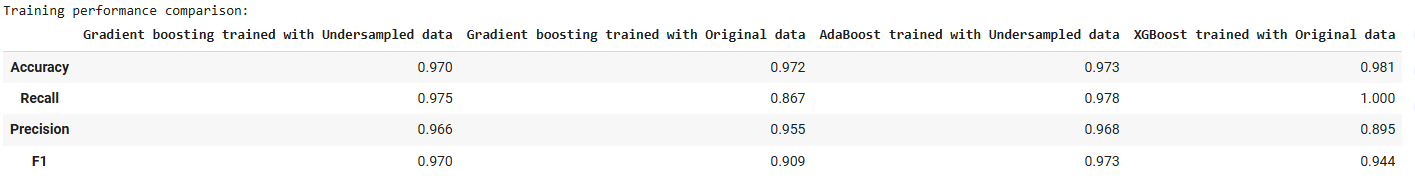
\includegraphics[width=\textwidth]{Training performance comparison.png}
		\caption{Training performance comparison.}
		\label{fig:Training performance comparison}
	\end{figure}
	\begin{figure}[h]
		\centering
		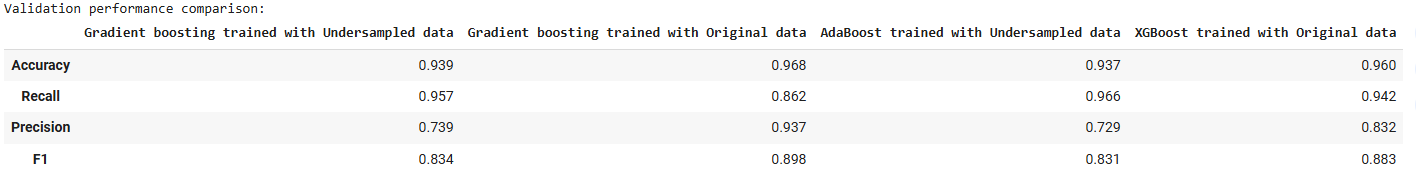
\includegraphics[width=\textwidth]{Validation performance comparison.png}
		\caption{Validation performance comparison.}
		\label{fig:Validation performance comparison}
	\end{figure}
	\begin{figure}[h]
		\centering
		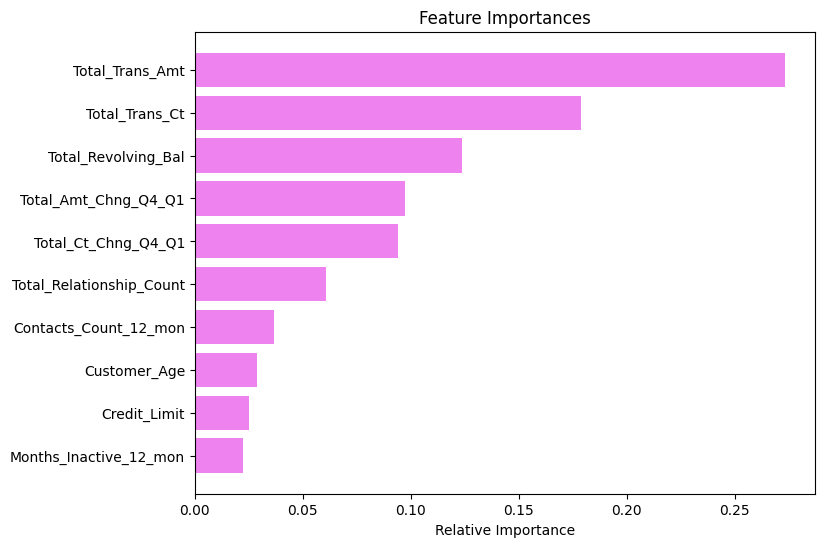
\includegraphics[width=0.7\textwidth]{feature_importance.png}
		\caption{Feature importance from final model(First 10).}
		\label{fig:feature_importance}
	\end{figure}
	For choosing the final model our motivation is primarily based on higher recall rate. But we se that for 2 point difference in recal  between AdaBoost trained with undersampled data and XGBoost trained with original data we have a trade of 11 points on the precision. If the 2 points difference in recall is heavier in terms of cost we should choose the AdaBoost trained with undersampled data. For now we recommend this model for the final one. But  XGBoost trained with original can also be used along side.
	
	On the test data set AdaBoost trained with undersampled data has following results on the metric : accuracy - 93.4 \%, Recall - 96.9\%, Precision - 71.8 \%, F1 - 82.5 \%. The Recall is very good which was our desire for the model building. Also since the test results are not very different from the validation set we can conclude that the model has done well generalization.
	
	We have shown in figure \ref{fig:feature_importance}, the feature importance generated from this final model for the first 10 features. We observe that Total trasaction amount has the highest weight/importance in determining attrition prediction.
	
\section{Actionable insights and Recommendations}
\subsection{Actionable insights}
\begin{enumerate}
	\setlength\itemsep{-2pt}
	\item There is 16\% total attrition rate in credit card service provided by thera bank. Since our focus is on retaining attriting customers. let's summarize the pattern among these customers.
	\item Customers with relationship count are more likely to attrition.
	\item Among 1,2 and 3 months of inactivity the probability of attrition increase from 1 to 3 with high confidence.
	\item Customers with higher contact count in last 12 months are more likely to attrit. 
	\item Females have slightly higher attrition ratio and the high earners ( more than 120K ) and low earners (less than 40K) have slightly higher attrition ratio.
	\item Attrited customers have significant lower median total transaction count and total transaction amount.
	\item Attrited customers generally have lower ratio of Q4 to Q1 transaction signifying that their transaction amount and count quarter over quarter has decreased.
	\item Attrited customers have lower median Average utilization ratio.
	\item After model building the Adaboost model trained with undersampled data has been shown to provide highest Recall of 96.9 \%. This is chosen as final  model.  
	\item Based on the final model, Total transaction amount, Total transaction count, Total Revolving Balance, Total Amount and count change Q4 to Q1 are five most important features which have highest weight in determining whether the customer will attrit. 
	\item Most of the credit card are type 'Blue'. There is very low preference among other types like 'platinum', 'silver', 'gold'.
\end{enumerate}

\subsection{Business Recommendations}
\begin{enumerate}
	\setlength\itemsep{-1pt}
	\item Make other services of bank highly attractive to customers as well to increase relationship count with the bank. Special efforts should be made to let customers know about all kinds of services from bank and it's benefits.
	\item More incentive can be give to females e.g cashback and offers during festival or Big billion days offer for reducing attrition rate among them. This apply to males as well.
	\item Total trasaction count and amount and quartely changes are very good predictors of attrition rate. Should these decline among any customers, they should be contacted by the agents via whats app or other online method for feedback. AI bots can also be used for these interaction based on the data on server.
	\item Take actions to diversify preference in credit card types. Customers are choosing 'Blue' type only. That means other types are not very attractive in features which needs improvement. At least study should be done on why those other types are not preferred among customers.
	\item Customers with 2 or 3 months of inactivity should be reminded by online method and their feed backs should be taken whether they are facing any issues.
	\item Use of Final model for decision making while credit card approval is recommended. 
\end{enumerate}
\begin{centering}
	\vspace{20pt}
	\subsection*{End of Report\\Submitted by : Haraprasad Dhal}
\end{centering}
\newpage
\section{Appendix}
\subsection{Further exploratory plots}
	\begin{figure}[h]
		\centering
		\begin{subfigure}[t]{0.47\linewidth}
			\centering
			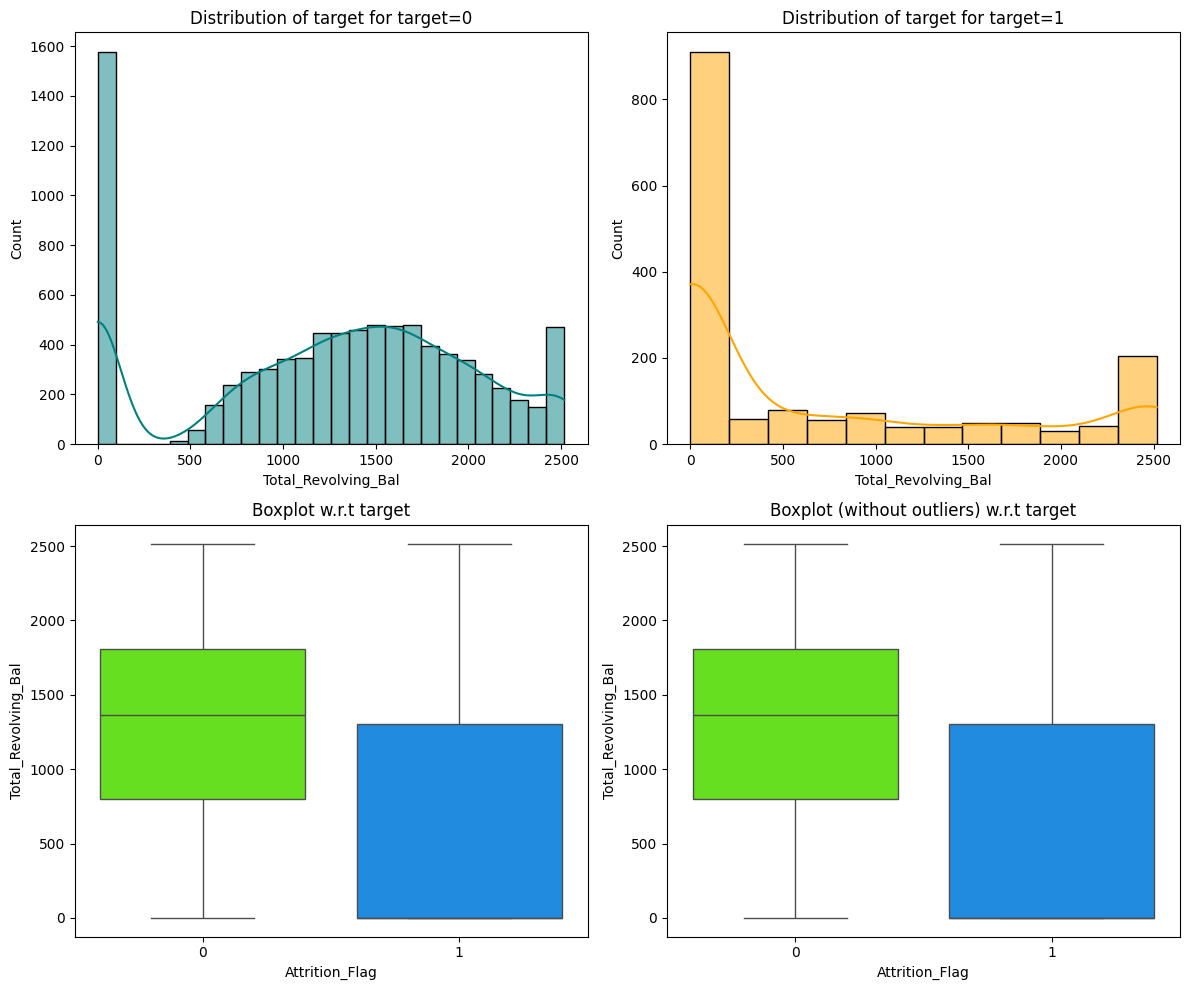
\includegraphics[width=\linewidth]{Total_Revolving_Bal vs Attrition_Flag.png}
			\caption{Histogram and boxplot of Total\_Revolving\_Balance w.r.t attrition flag}
			\label{fig:Total_Revolving_Bal vs Attrition_Flag}
		\end{subfigure}
		\hfill
		\begin{subfigure}[t]{0.47\linewidth}
			\centering
			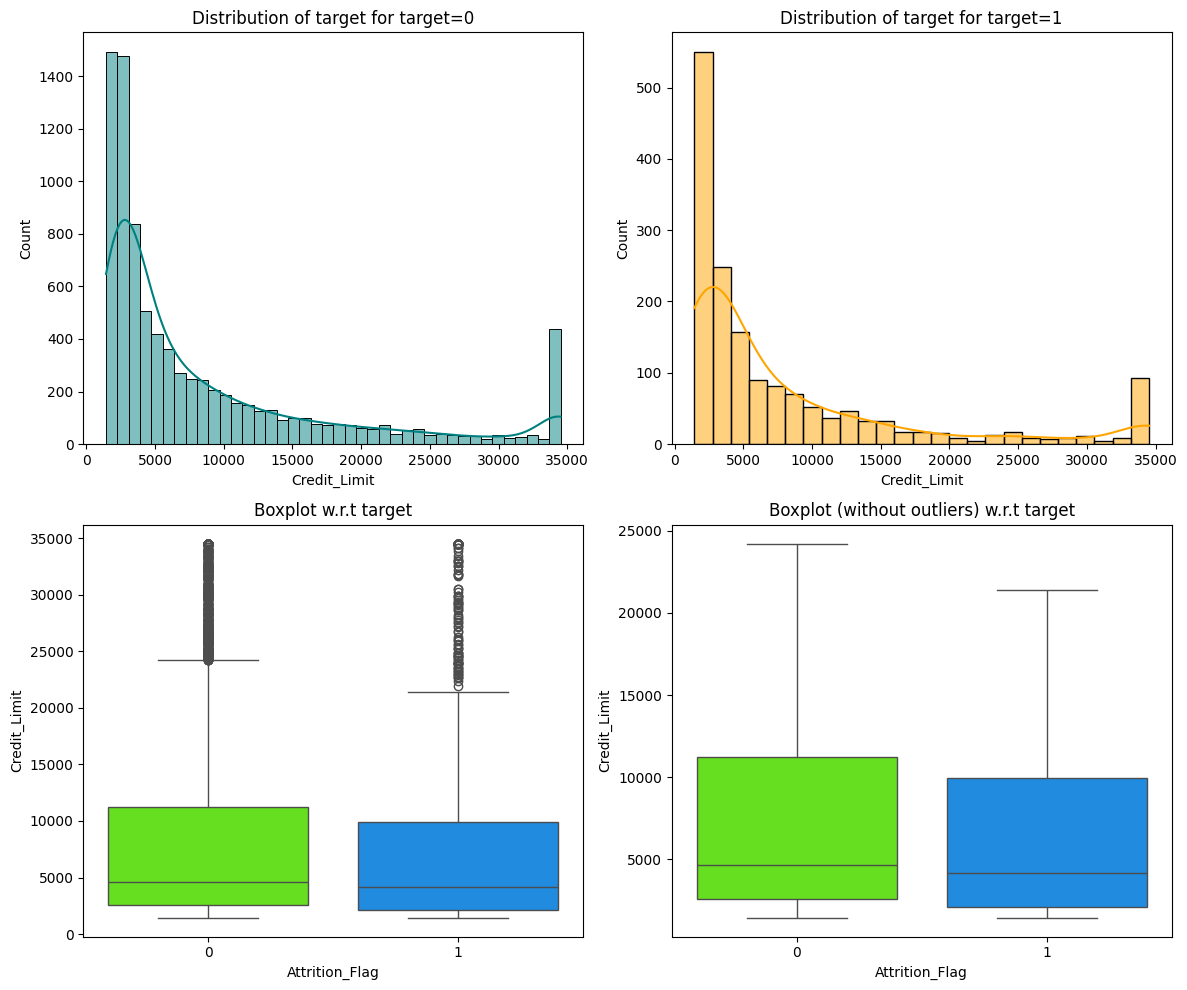
\includegraphics[width=\linewidth]{Attrition_Flag vs Credit_Limit.png}
			\caption{Histogram and boxplot of Credit\_Limit amount w.r.t attrition flag}
			\label{fig:Attrition_Flag vs Credit_Limit}
		\end{subfigure}
		\hfill
		\begin{subfigure}[t]{0.47\linewidth}
			\centering
			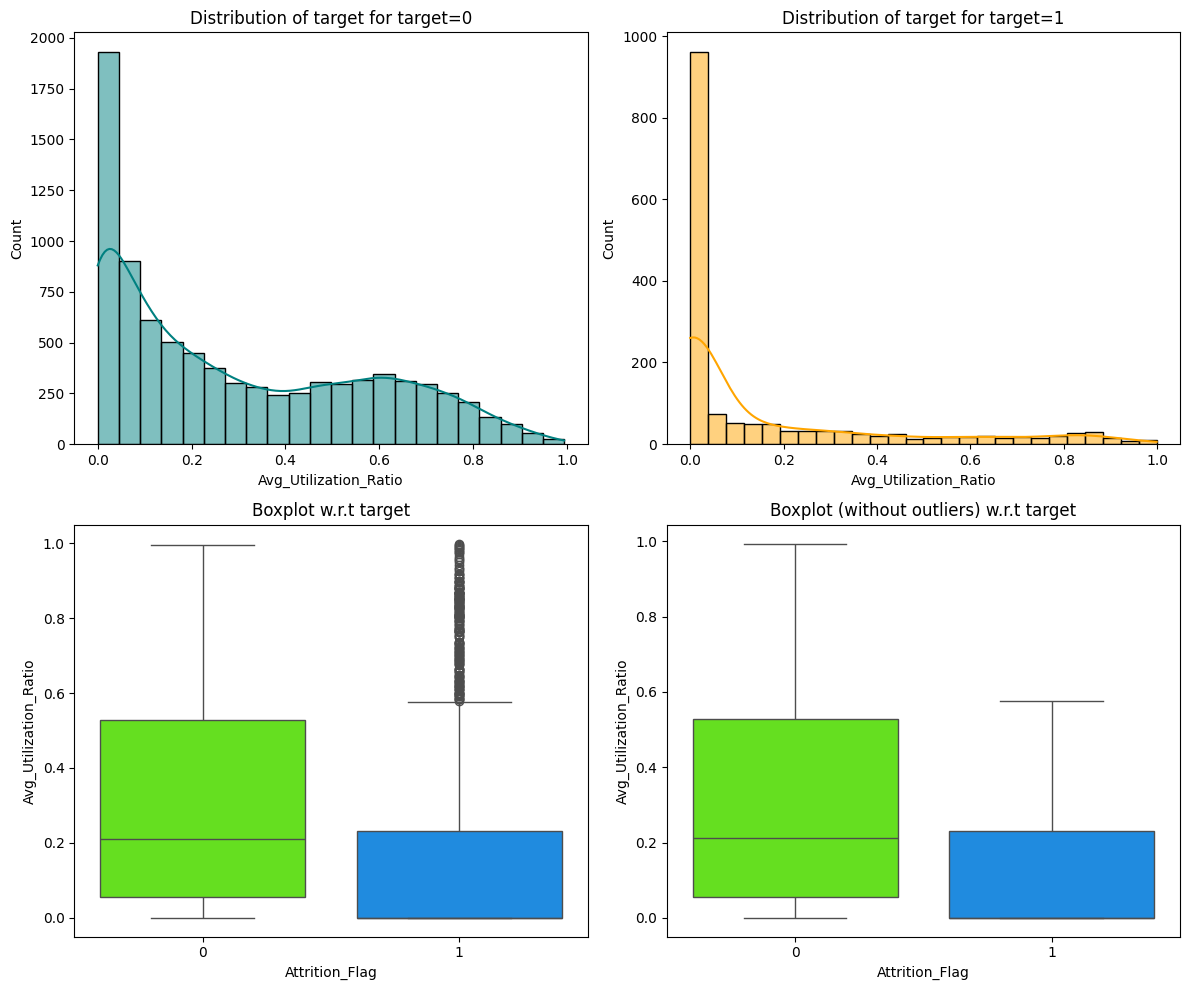
\includegraphics[width=\linewidth]{Avg_Utilization_Ratio vs Attrition_Flag.png}
			\caption{Histogram and boxplot of Avg\_Utilization\_Ratio w.r.t attrition flag}
			\label{fig:Avg_Utilization_Ratio vs Attrition_Flag}
		\end{subfigure}
		\hfill
		\begin{subfigure}[t]{0.47\linewidth}
			\centering
			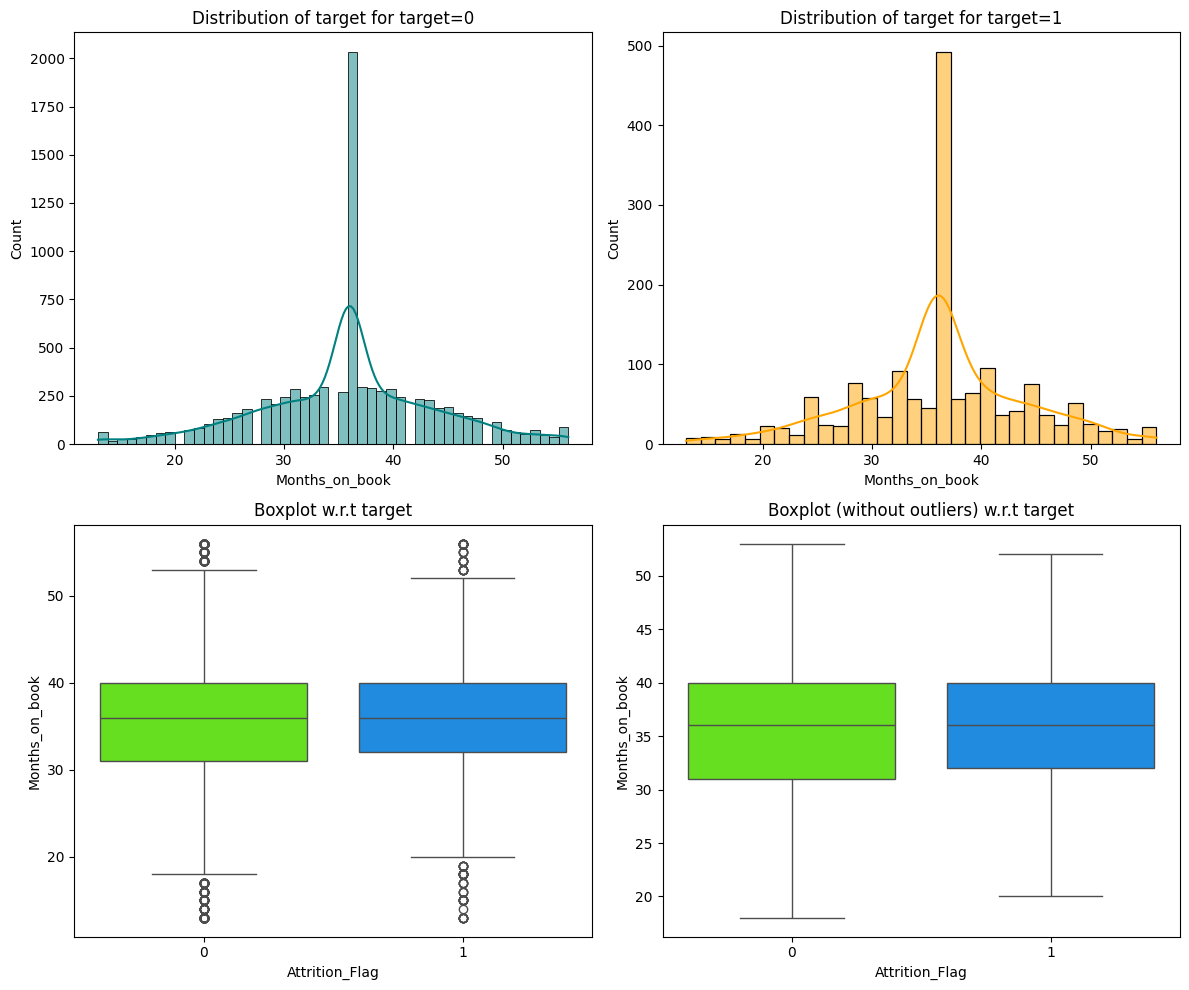
\includegraphics[width=\linewidth]{Attrition_Flag vs Months_on_book.png}
			\caption{Histogram and boxplot  Months\_on\_book w.r.t attrition flag}
			\label{fig:Attrition_Flag vs Months_on_book}
		\end{subfigure}
		\caption{Distribution of numerical variables with respect attrition flag}
		\label{fig: Distribution of further numerical variables with respect attrition flag}
	\end{figure}
	
	\begin{figure}[h]
		\centering
		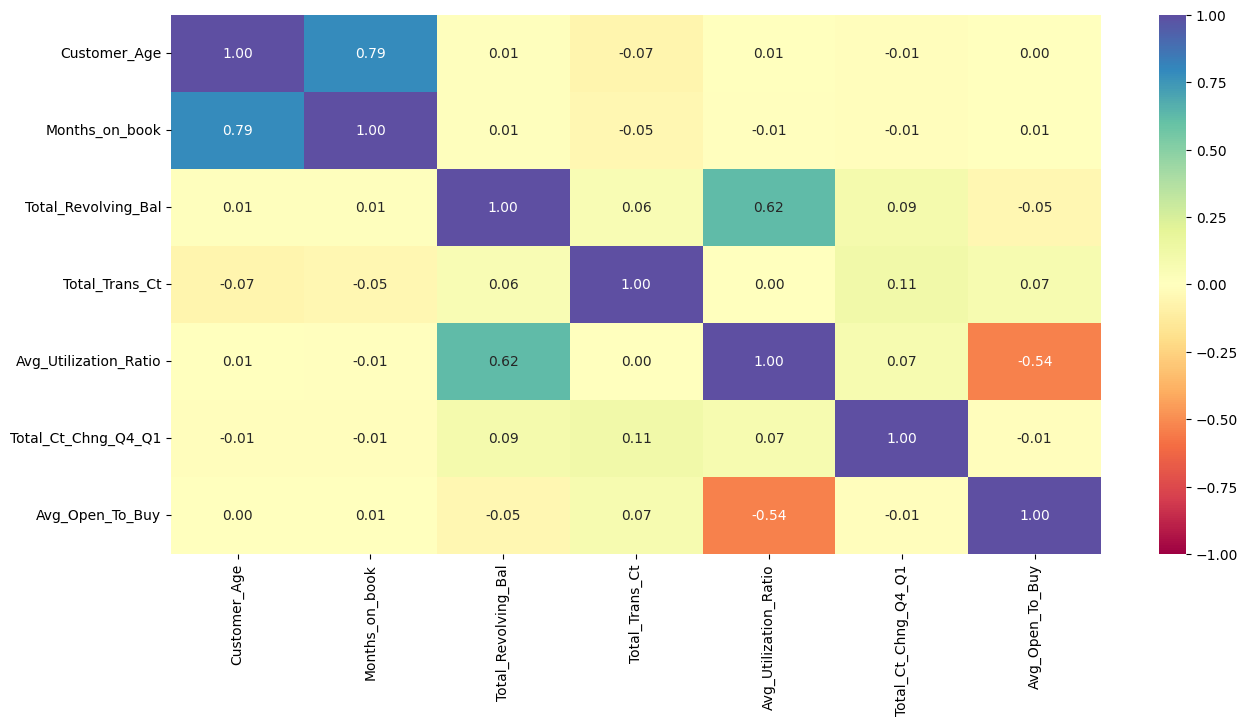
\includegraphics[width=0.8\textwidth]{corr.png}
		\caption{Correlation among numerical variables.}
		\label{fig:corr}
	\end{figure}
	
	
\end{document}